\section{Introduction to Project}
\begin{figure}[!ht]
\centering
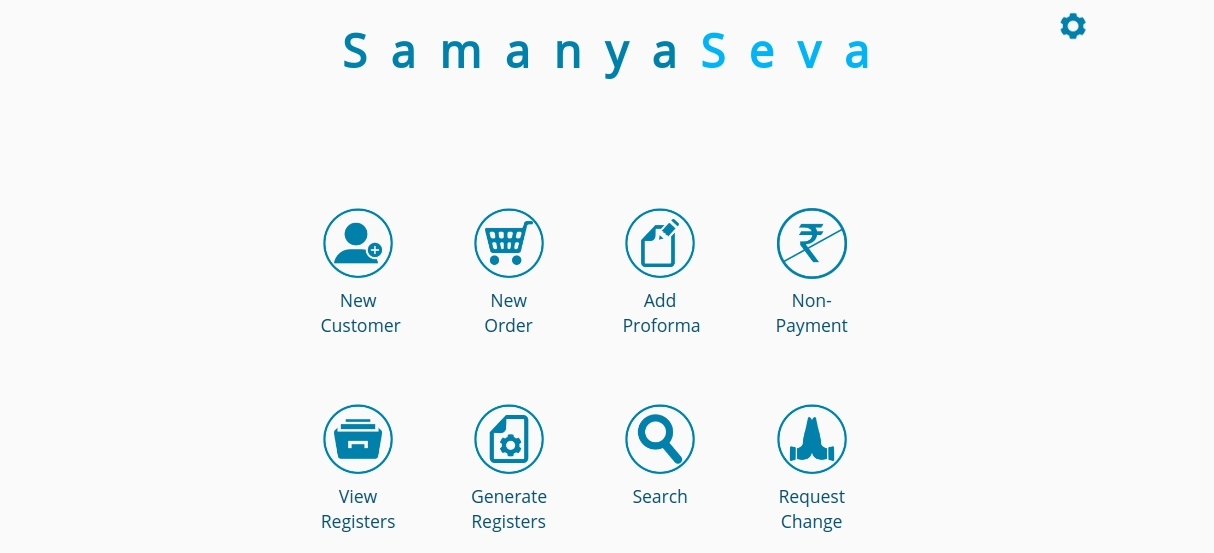
\includegraphics[scale=0.41]{input/images/samanya1.png}                   
\caption{Client Management Assure}
\hspace{-1.5em}
\end{figure}
\subsection{What is SamanyaSeva?}
 SamanyaSeva is an integrated software solution offered which can be used to support the seamless integration of information that flows through an organization. The basic idea was to make a generalized E-commerce software. It is provided as a package comprising different modules, such as Bills, Voucher, Catalog, Customer information etc.\\
 Mainly, a SamanySeva software is a customer relationship management tool that most businesses use to manage and analyze customer interactions and data throughout the customer lifecycle, with the goal of improving business relationships with customers, assisting in customer retention and driving sales growth.\\\\
It is basically an E-Commerce cum CRM (Customer relationship management) Django Web Application.
The basic idea behind it was to make a generalized E-commerce software that could be implemented in Companies as well as hospitals, bakery and other shops.\\\\
This project is basically a combination of people, processes and technology that seeks to understand a company's customers. It is an integrated approach to managing relationships by focusing on customer retention and relationship development. In code, there are several modules in SamanyaSeva including Catalog, Reports, Bills, Prints, Program Letter, Voucher.\\\\
CRM revolves around people, process and technology. SamanyaSeva has been developed using the latest technologies. Earning profit is the principal and final goal of any commercial activity. Being a catalyst for interplay with clients, CRM aids the earning power enhancement. 

\subsection{Who uses SamanyaSeva}
Customer Relation Management systems are widely used by engineering teams and scientists, in both industry and academia
for different purposes. Its even been used by business maintenance teams and various authors, for attract-
ing the crowd and for promoting their work. 
These can be used in various sectors:
\begin{itemize}
	\item Business Sector
	\item Education Sector
	\item IT firms
	\item Organizations
\end{itemize}

\subsection{Why SamanyaSeva?}
The reason why we thought of creating a CRM system of our own because we wanted to get a very specific idea
of what it should do, and how it should work. These systems are a necessity nowadays
for business areas. SamanyaSeva can provide service in many fields and can maintain the record with an ease. It enhances the productivity of business.
Some of it's benefits:
\begin{itemize}
	\item Improved Information arrangement
	\item  Enhance Productivity
	\item Improved Customer Support
	\item Task Automation
	 \item Team Work Efficiency
	 \item Improved Reporting \& Analysis
\end{itemize}

\section{Project Category}
Categories and category groups are organized by types. These types correspond to the transaction types that are available in Project management and accounting.\\
SamanyaSeva comes under the category of Application or System Development. The project mainly falls under the domain of Industry Oriented. 

\section{Objective of Project}
SamanyaSeva is a CRM cum ERP Application and the 
main objectives of this project is to :
\begin{enumerate}
\item Enhancing the operational efficiency of business resources. 
\item To make an open source project in which people can contribute and learn.
\item To follow modular approach for easy configuration.
\end{enumerate}

\section{Problem Formulation}
As the market is rising rapidly, so is the demand and technology. SamanyaSeva will provide a platform to business oriented marketers, Education Sectors etc. to store their important data at a single place which provides alot of benefits. The USP of this project will be it's modular approach and catalogue.

\section{Need and Significance}
\begin{itemize}
\item Better customer satisfaction.
	\item Improved supplier Performance.
	\item Improved Resource Utility.
\end{itemize}

\section{The Existing System}
There are few existing systems which do the task like Busy, SAP or other softwares but
they don't have few features which are here in this system. Migration of existing data to the new ERP systems is difficult (or impossible) to achieve. Integrating ERP systems with other stand alone software systems is equally difficult (if possible). These activities may consume a lot of time, money \& resources. Moreover, these system were not open source and free web based software. SamanyaSeva uses Django which makes it easier to migrate from one type of database to other.
All exiting systems suffers from at least one of the following:
 \subsection{Limitations of previous system }
\begin{itemize}
\item No Modular Approach. 

\item No Independent modules such as Catalog.

\item Can't be easily configured for different purposes.


\end{itemize}
\section{Technologies Used}
\begin{enumerate}
\item Web Development languages (JS, HTML, CSS)
\item Django (Python Framework)
\item Bootstrap
\item MySQL
\item Apache
\item Hovercraft
\item LaTeX
\item Git

\end{enumerate}

\section{Unique Features of Proposed System}
\begin{itemize}
	\item Modular Approach
	\item Proper Catalog
	\item Easy Configuration
	\item Independent Modules
	\end{itemize}

\newpage


